\documentclass[aspectratio=169]{beamer}
\usepackage[utf8]{inputenc}
\usepackage{tikz} % For semi-transparent background blocks
\usepackage{hyperref}
\usepackage{multimedia}
\usepackage{ulem}
\usepackage{wasysym}

\usepackage{pbox}

\usepackage[absolute,overlay]{textpos}

\usepackage{smartdiagram}
\usetikzlibrary{shapes.geometric,calc}
\usetikzlibrary{shapes.symbols}
\usetikzlibrary{shapes.symbols,positioning}
\usepackage{metalogo}

\usetikzlibrary{backgrounds, calc, shadows, shadows.blur}

\newcommand\addcurlyshadow[2][]{
    % #1: Optional aditional tikz options
    % #2: Name of the node to "decorate"
    \begin{pgfonlayer}{background}
        \path[blur shadow={shadow xshift=0pt, shadow yshift=0pt, shadow blur steps=6}, #1]
        ($(#2.north west)+(.3ex,-.5ex)$)
        -- ($(#2.south west)+(.5ex,-.7ex)$)
        .. controls ($(#2.south)!.3!(#2.south west)$) .. (#2.south)
        .. controls ($(#2.south)!.3!(#2.south east)$) .. ($(#2.south east)+(-.5ex,-.7ex)$)
        -- ($(#2.north east)+(-.3ex, -.5ex)$)
        -- cycle;
    \end{pgfonlayer}
}

%%%%%%%%%%%%%%%%%%%%%%%%%%%%%%%%%%%%%%%%%%%%%%%%%%%%%%%%%%%%%%%%%%%
% Style modifications
%%%%%%%%%%%%%%%%%%%%%%%%%%%%%%%%%%%%%%%%%%%%%%%%%%%%%%%%%%%%%%%%%%%

\usetheme{Berlin}

%%% Fonts %%%

% Change font. Fontspec requires xelatex instead of pdflatex!
% Font catalog: http://www.tug.dk/FontCatalogue/
\usepackage{fontspec}

%\setsansfont{Comfortaa}
%\setsansfont{DejaVu Sans}
%\setsansfont{Fira Sans}

% Use "Fira Sans Light" as the normal font and the "Fira Sans" for
% bold fonts

\setsansfont[
  ItalicFont={Fira Sans Light Italic},
  BoldFont={Fira Sans},
  BoldItalicFont={Fira Sans Italic}]{Fira Sans Light}

\setbeamerfont{title}{size=\Large, series=\bfseries}
\setbeamerfont{frametitle}{size=\large, series=\bfseries}

%%% Slide template %%%

\setbeamertemplate{frames}[default]

% Empty headline / footline
\setbeamertemplate{headline}{}
\setbeamertemplate{footline}{}

% Remove navigation icons
\setbeamertemplate{navigation symbols}{}

%%% Colors %%%

\usecolortheme{crane}

\definecolor{lightgray}{RGB}{220,220,220}
\definecolor{darkgray}{RGB}{45,45,45}
%\definecolor{darkblue}{RGB}{0,86,137}
%\definecolor{darkblue}{RGB}{22,90,151}
\definecolor{lightblue}{RGB}{229, 245, 255}

%\definecolor{darkblue}{RGB}{1,1,100}


% Use the slide background in block environments                                                                                                      
\setbeamercolor{title}{fg=white,bg=darkgray}
\setbeamertemplate{blocks}[default]
\setbeamercolor{block title}{bg=}
\setbeamercolor{block body}{bg=lightgray}
\setbeamercolor{frametitle}{fg=white,bg=darkgray}
\setbeamerfont{block body}{size=\large}
\setbeamercolor{itemize item}{fg=black}
\setbeamertemplate{itemize items}[circle]
\setbeamercolor{section number projected}{bg=darkgray,fg=white}
\setbeamercolor{section in toc}{fg=black}
\setbeamercolor{subsection in toc}{fg=darkgray}

\addtobeamertemplate{block begin}{\pgfsetfillopacity{0.8}}{\pgfsetfillopacity{1}}
\addtobeamertemplate{frametitle}{\pgfsetfillopacity{1.0}}{\pgfsetfillopacity{1}}
\addtobeamertemplate{title page}{\pgfsetfillopacity{1.0}}{\pgfsetfillopacity{1}}

%%% Misc %%%

% Command to place the test (e.g. citation) in the center of the footer
\newcommand{\setfootercentertext}[1]{
\setbeamertemplate{footline}{
  \hspace*{\fill}
  \raisebox{3mm}[0mm][0mm]{
    \tiny{#1}}\hspace*{\fill}}
}

%%%%%%%%%%%%%%%%%%%%%%%%%%%%%%%%%%%%%%%%%%%%%%%%%%%%%%%%%%%%%%%%%%%
% Content
%%%%%%%%%%%%%%%%%%%%%%%%%%%%%%%%%%%%%%%%%%%%%%%%%%%%%%%%%%%%%%%%%%%

%------------------------------------------------------------------------------
\title{Visualization basics for \\data exploration and communication}
%------------------------------------------------------------------------------

\author{\small Prof. Dr. Konrad U. Förstner}

%\institute{ZB MED -- Information Center Life Sciences, Cologne, Germany \&\\
%  TH Köln -- University of Applied Sciences, Cologne Germany}

\date{\scriptsize
  Virtual Summer School \textit{Data Literacy in Health}, August 26 2021\\ \ \\
  % \includegraphics[width=1.0cm]{images/vcard_qr_code.png}\ \\ \ \\
  
\includegraphics[width=1.0cm]{images/creative_commons_attribute.png}
}

\logo{
  
\includegraphics[height=1.0cm]{images/ZBMED_2017_EN.pdf}
  
\includegraphics[height=0.8cm]{images/logo_TH-Koeln_CMYK_22pt.eps}
}


\begin{document}


\begin{frame}{}
  \titlepage
\end{frame}
\logo{}


\setbeamertemplate{background}{}
\setbeamertemplate{footline}{}

\setbeamertemplate{background}{}
\setfootercentertext{}
\begin{frame}
  \frametitle{}
  \begin{center}
    Slides and Code (Jupyter Notebooks) can be found here:\\
    \ \\
    \includegraphics[width=3cm]{images/qr_to_git_repo.eps}\\
    \ \\
    \href{https://github.com/foerstner-lab/2021-08-26-Visualisation_basics_for_data_exploration_and_communication}{https://github.com/foerstner-lab/2021-08-26-Visualisation\_basics\_for\_data\_exploration\_and\_communication}\\
    \ \\
    \href{https://bit.ly/2XODDoM}{https://bit.ly/2XODDoM}
  \end{center}

\end{frame}

\setbeamertemplate{background}{}
\setfootercentertext{}

\begin{frame}
  \frametitle{Plan for this session}
  \begin{center}
    {\LARGE
    \begin{tabular}{lll}
      09:00 - 10:00 & Introduction \& Live Coding\\
      10:00 - 11:00 & Working on your data\\
      11:00 - 12:00 & Discussion, Questions \& Answers\\
    \end{tabular}
    }
  \end{center}
\end{frame}


\begin{frame}
  % \frametitle{Basic concept of supervised machine learning}
  \begin{block}{}
    \vspace{0.5cm}
    \ \ \ \
    \begin{minipage}{0.10\textwidth}
      \begin{center}
        
\includegraphics[width=1.6cm]{images/publicdomainvectors_target-plain.pdf}
      \end{center}        
    \end{minipage}
    \hfill
    \begin{minipage}{0.80\textwidth}
      After this session you should have a basic understanding of
      selected concepts of data visualization that are independent
      of the tool that you use.
    \end{minipage}
    \vspace{0.3cm}
  \end{block}
\end{frame}

%%%%%%%%%%%%%%%%%%%%%%
\section{Introduction \& Live Coding}
%%%%%%%%%%%%%%%%%%%%%%

\begin{frame}{}
 \tableofcontents
\end{frame}

\begin{frame}{}
  \tableofcontents[currentsection]
\end{frame}

\setbeamertemplate{background}{
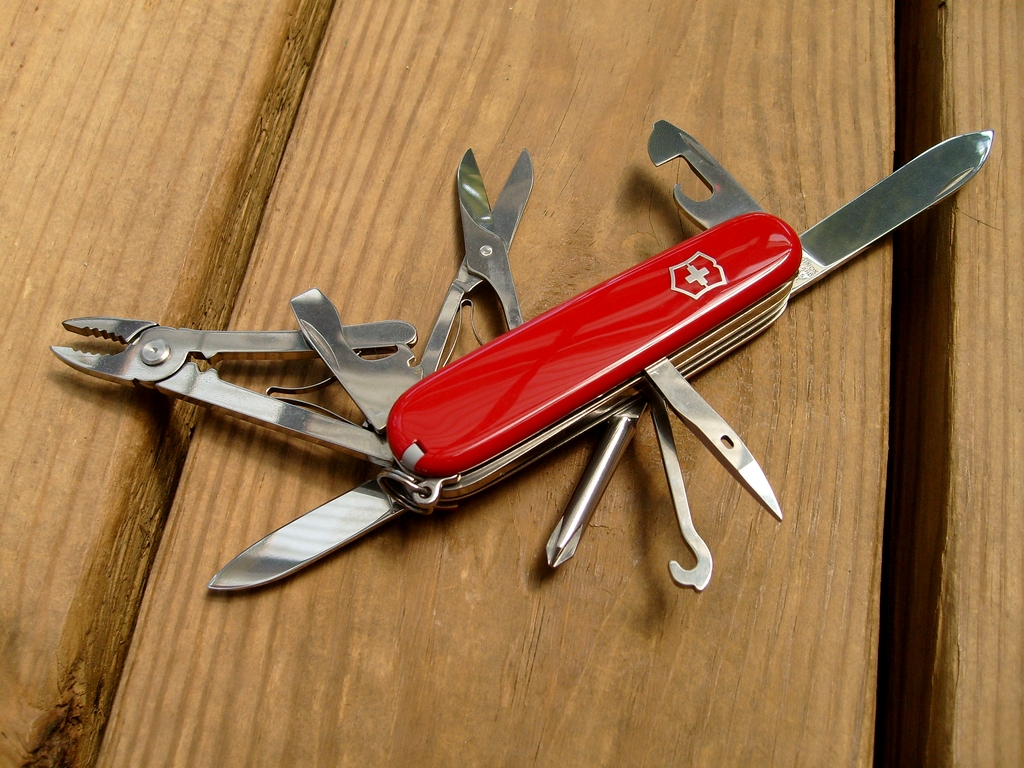
\includegraphics[width=\paperwidth]{images/flickr_capcase_4970062156_Swiss_Army_Knife.jpg}}
\setbeamertemplate{footline}{\raisebox{2mm}[2mm][2mm]{\Tiny{\
       \href{https://www.flickr.com/photos/capcase/4970062156/}{https://www.flickr.com/photos/capcase/4970062156/}
      -- CC-BY by flickr user \href{http://www.flickr.com/photos/capcase/}{capcase}}}}
\begin{frame}
  % \frametitle{A swiss army knife for systems biology}
  \begin{block}{}
    \begin{center}
      Visualisation are powerful tools to \\understand data and
      communicate ideas.
    \end{center}
  \end{block}
\end{frame}
\setbeamertemplate{background}{}
\setbeamertemplate{footline}{}

\setbeamertemplate{background}{}
\setfootercentertext{}
\begin{frame}
  \frametitle{Visualising ideas, plans or concepts}
  \begin{center}
    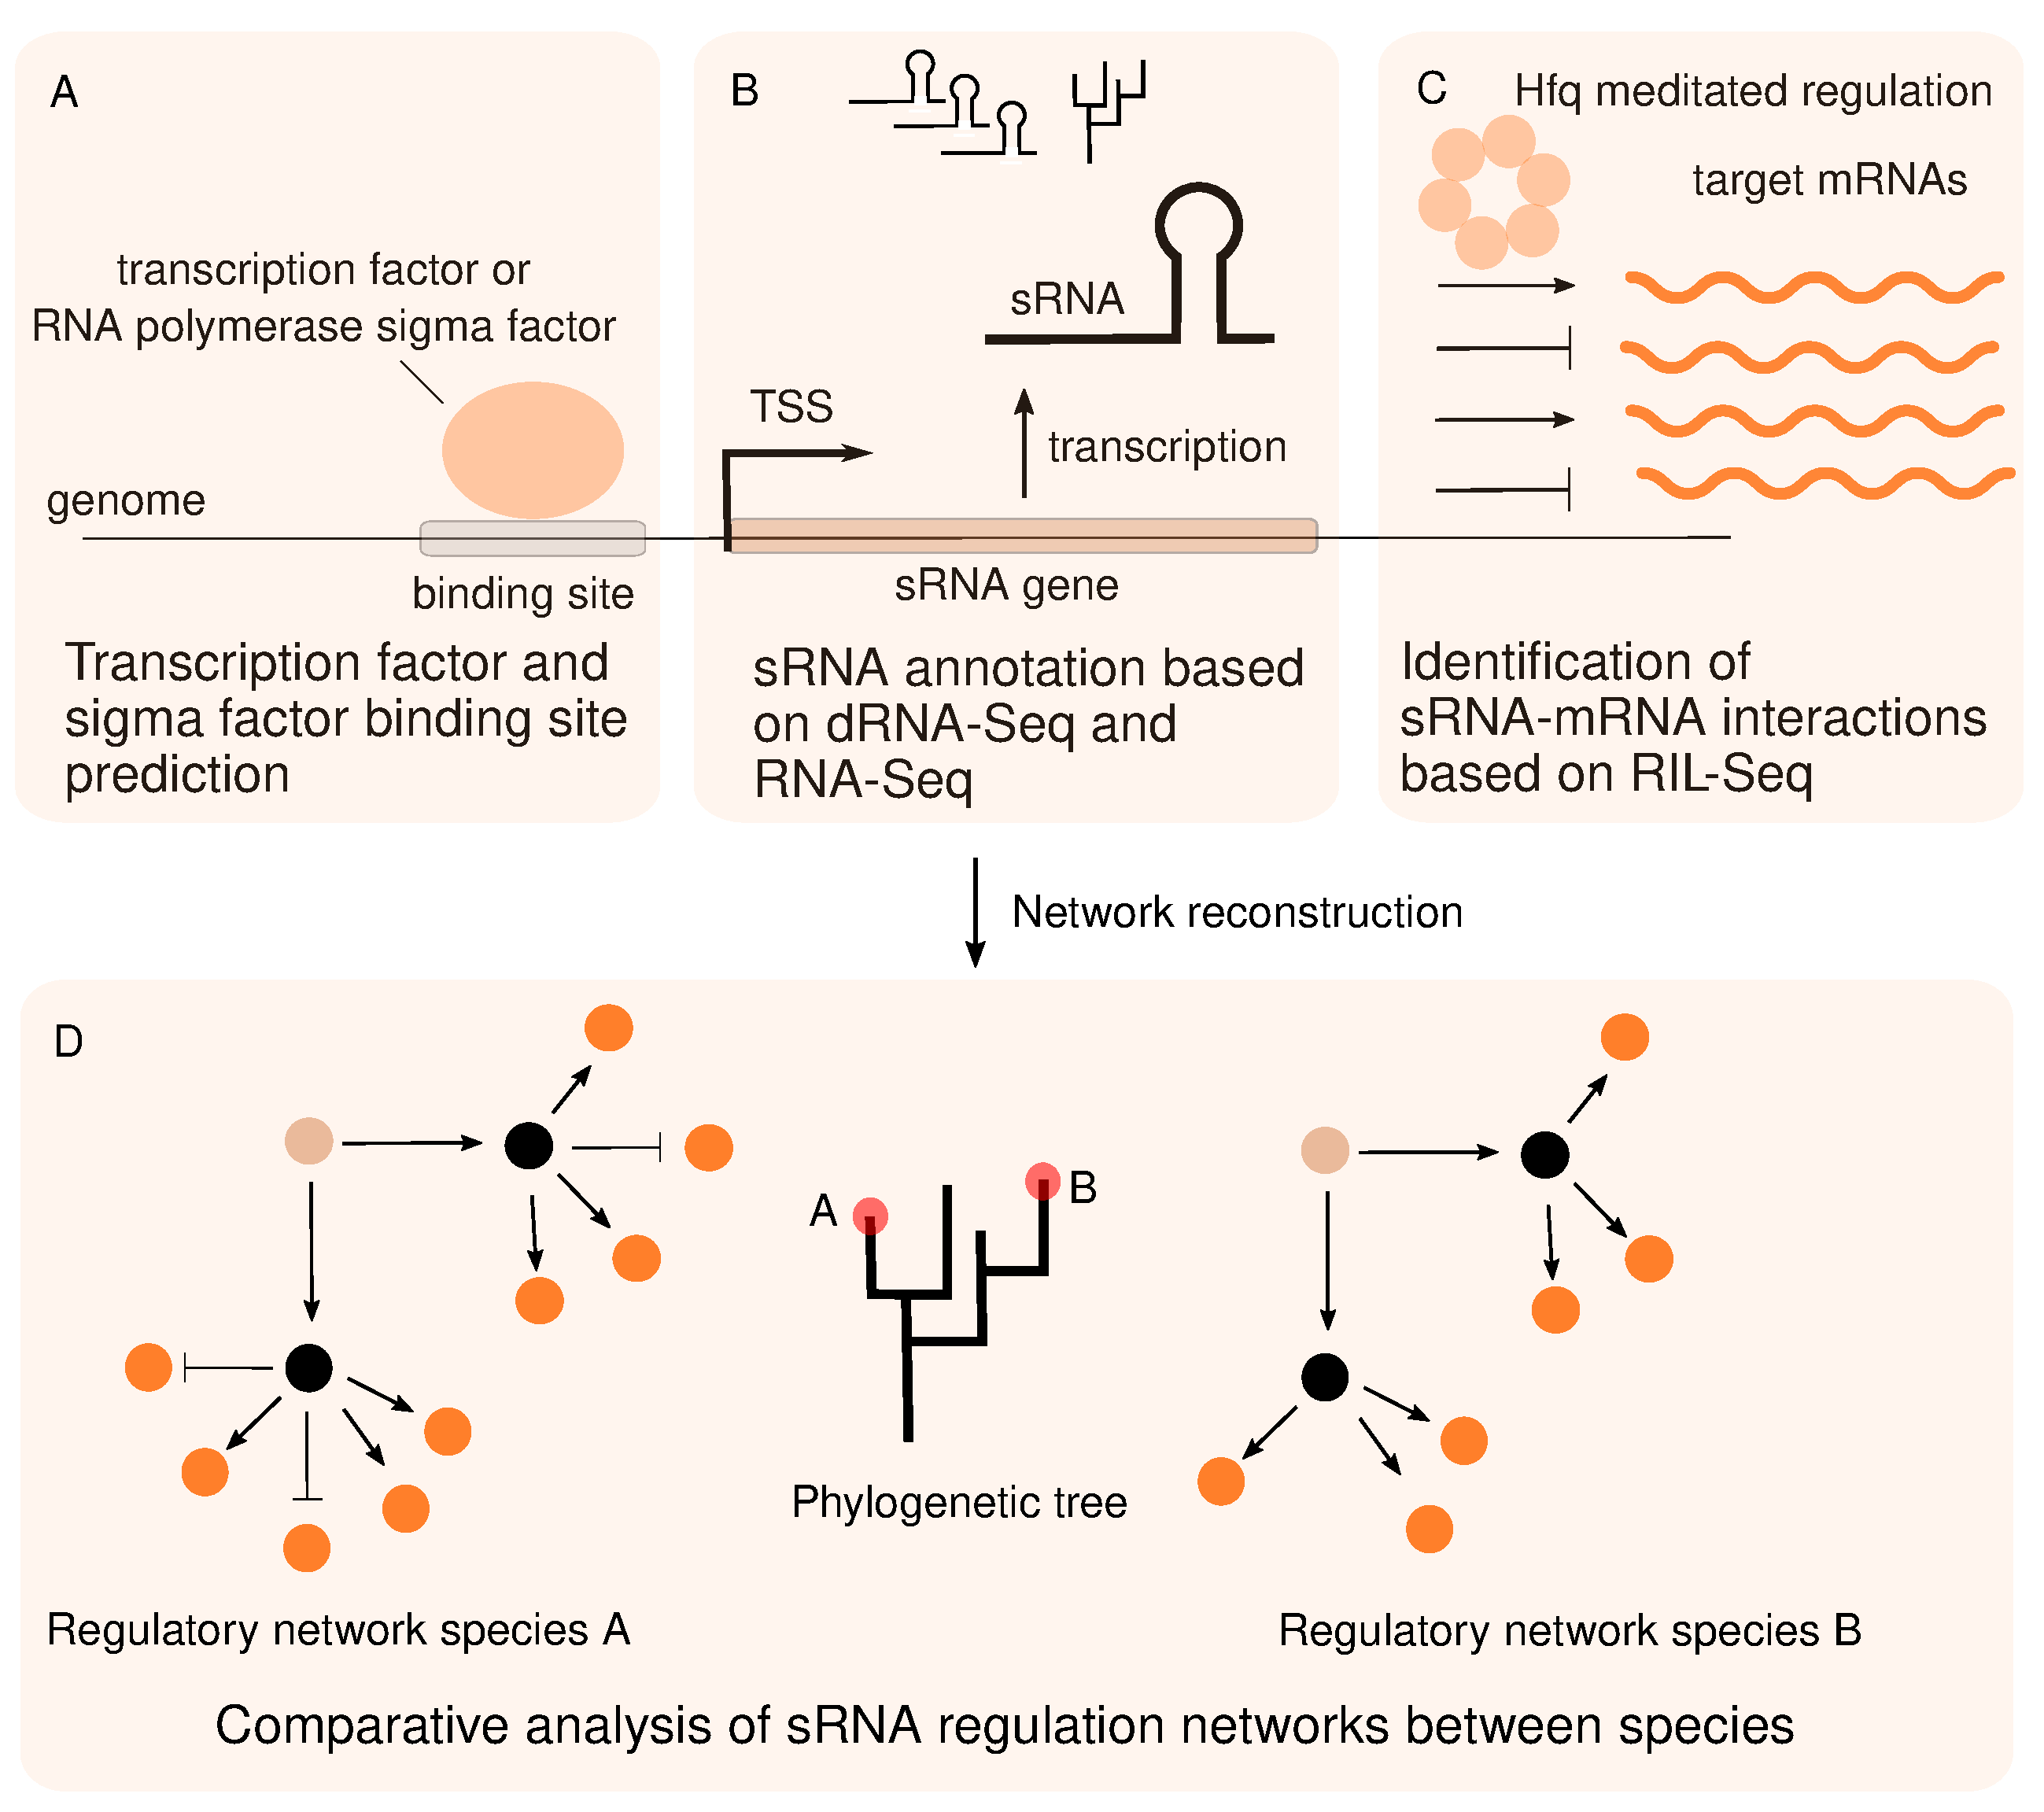
\includegraphics[width=8.5cm]{images/sRNARegNet_Working_plan.pdf}\\
  \end{center}
\end{frame}


\setfootercentertext{
  Berger, \textit{et al.}, 2016, \textit{Sci. Rep.},
  \href{https://doi.org/10.1038/srep35307}{https://doi.org/10.1038/srep35307}
}
\begin{frame}{}
  \frametitle{Visualising research results}
  \begin{center}
    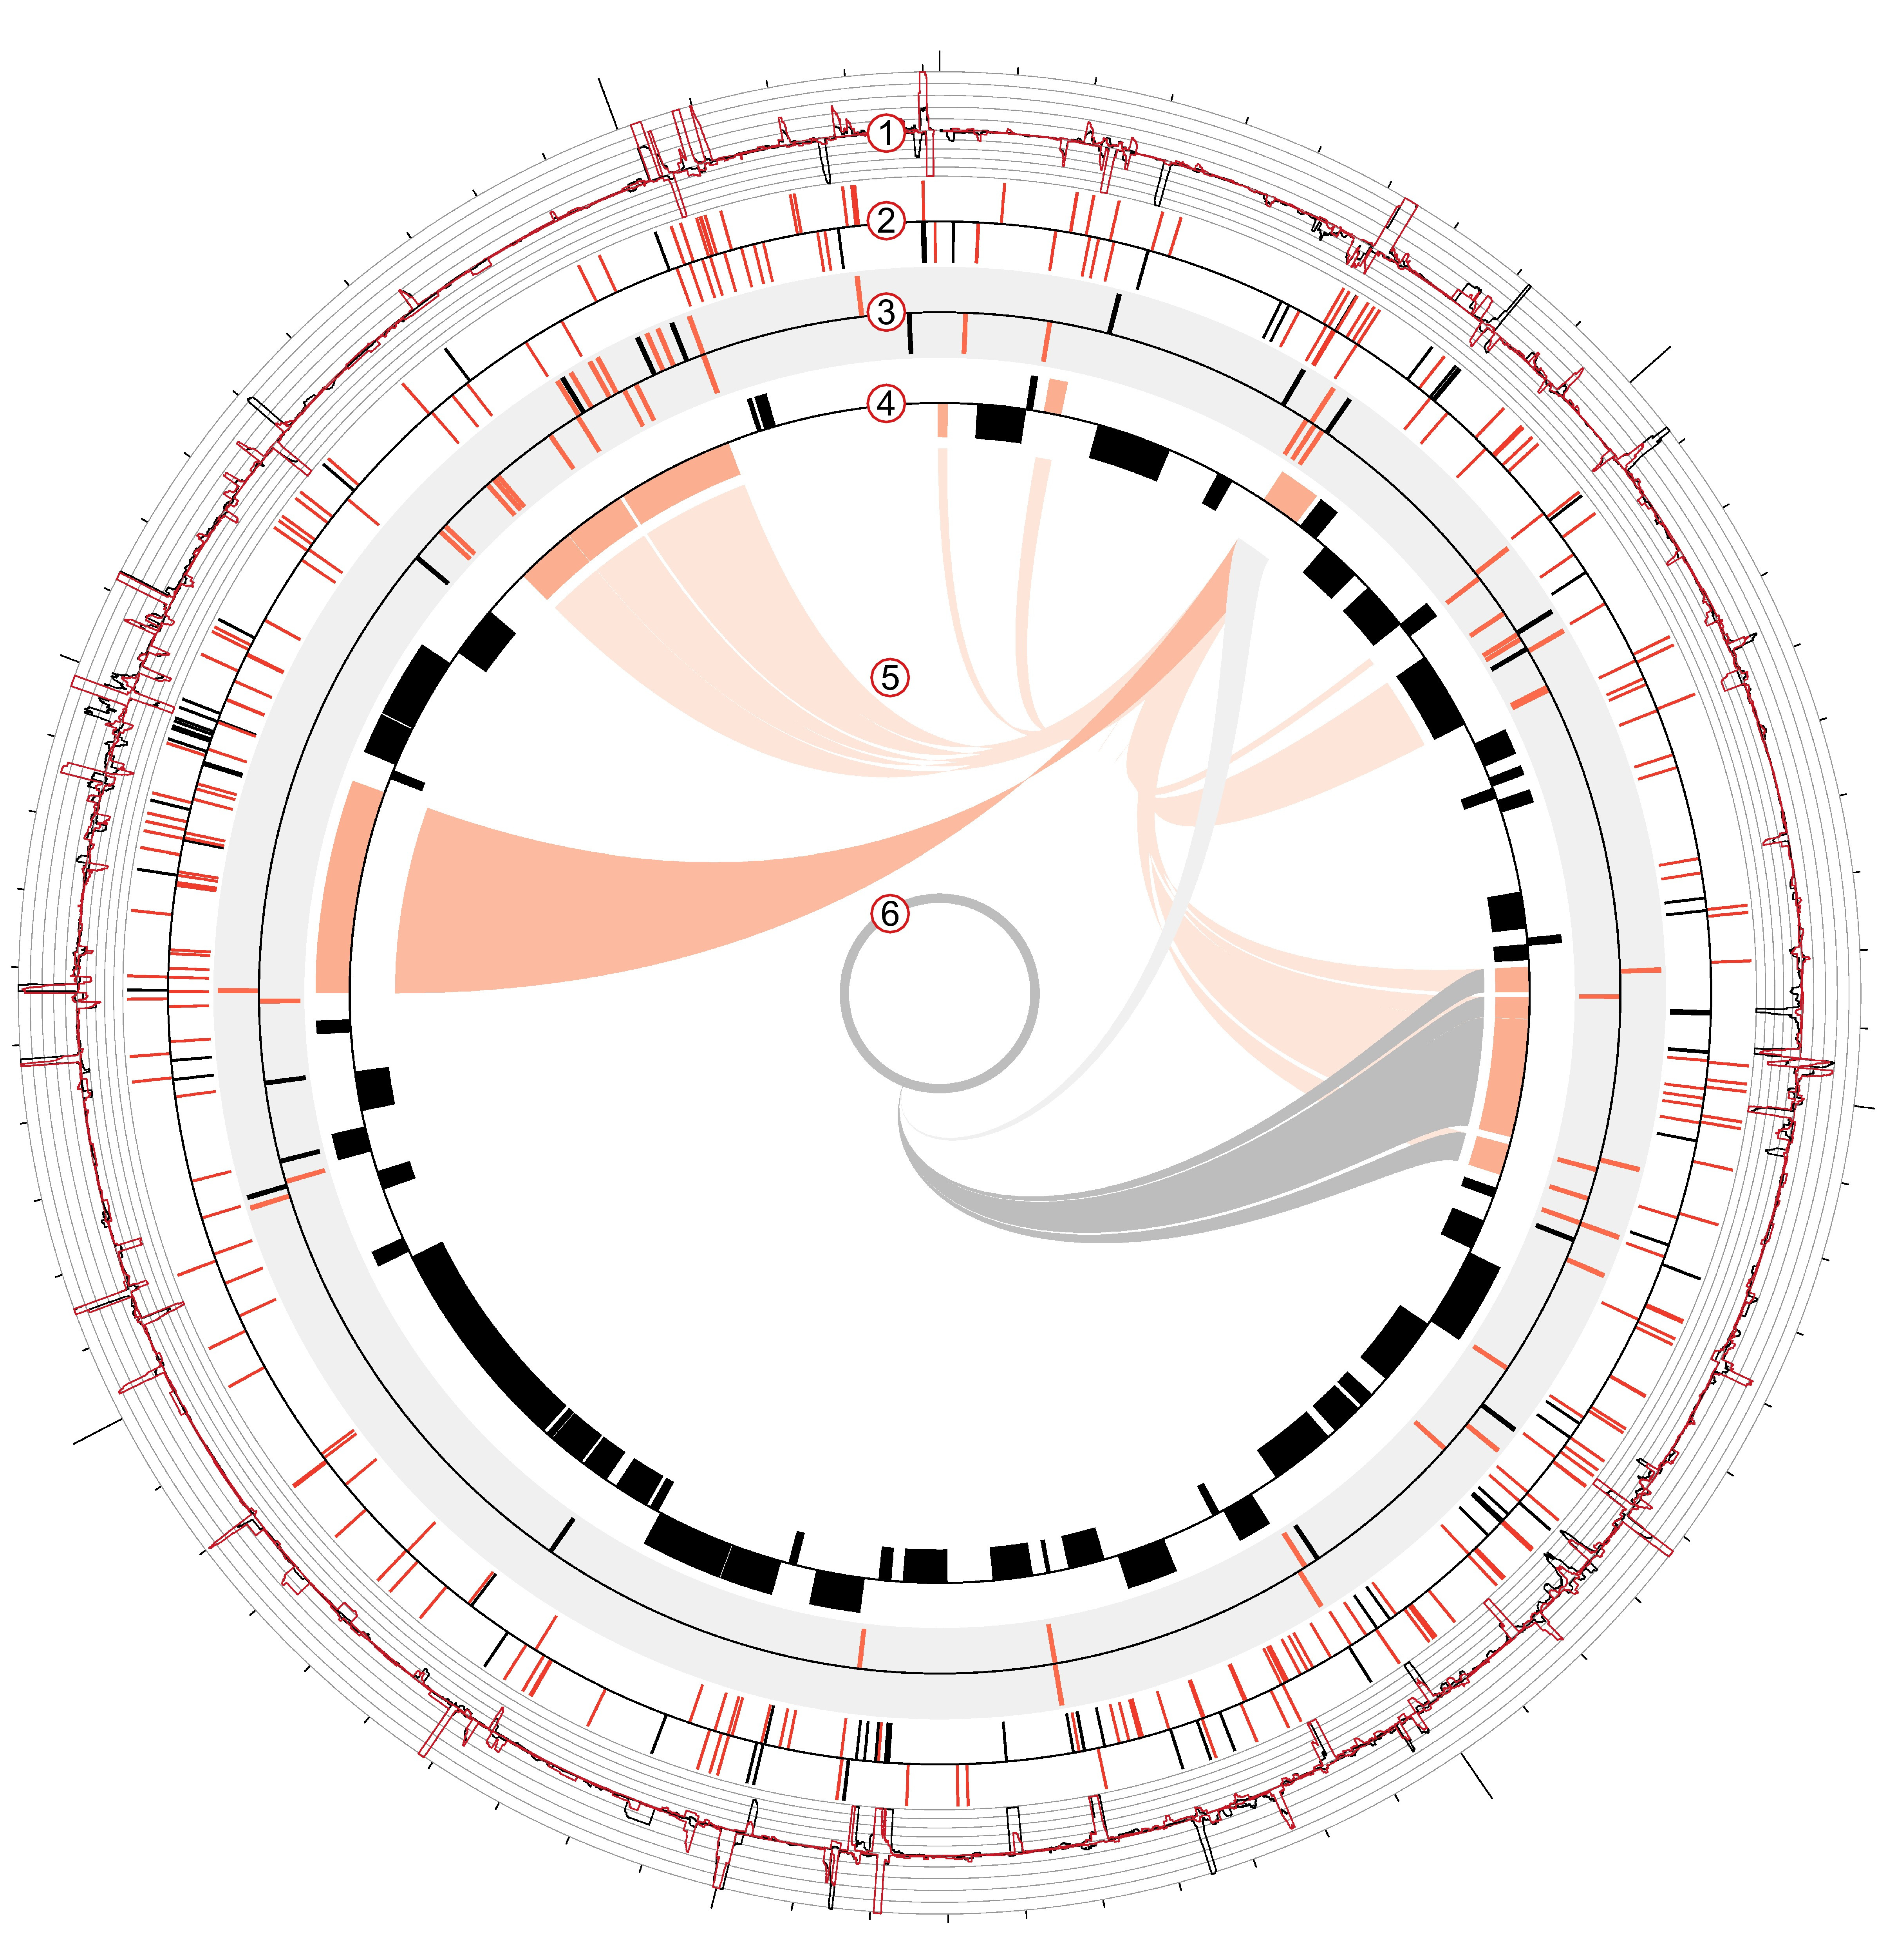
\includegraphics[height=5.5cm]{images/Berger_Knoedler_Foerstner_et_al_Fig_1.jpg}\\
  \end{center}  
\end{frame}

\setbeamertemplate{background}{}
\setfootercentertext{}
\begin{frame}
  %\frametitle{Visualising ideas, plans or concepts}
  \begin{center}
    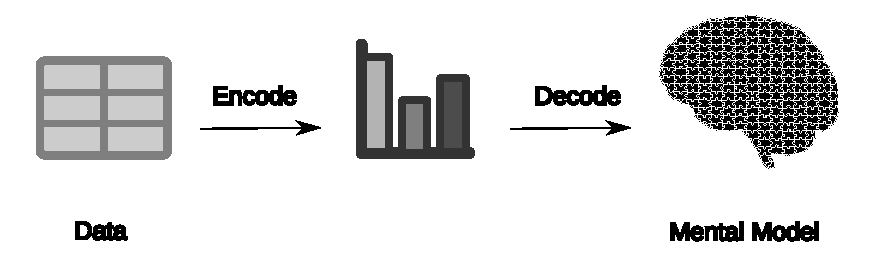
\includegraphics[width=12cm]{images/Data_encode_visualisation_decode.pdf}\\
  \end{center}
\end{frame}

\begin{frame}
  \frametitle{Entities and their features}    
  \begin{block}{}
    \vspace{0.5cm}
    \ \ \ \
    \begin{minipage}{0.10\textwidth}
      \begin{center}
        
\includegraphics[width=1.6cm]{images/publicdomainvectors_ftdissociatecell.pdf}
      \end{center}        
    \end{minipage}
    \hfill
    \begin{minipage}{0.80\textwidth}

      Features can be\\
      \begin{itemize}
        \item categorical / qualitative
          \begin{itemize}
          \item Nominal (e.g. cell line, cancer type, eye color, gender)
          \item Ordinal (e.g. very bad, bad, good, very good)
          \end{itemize}
        \item numerical / quantitative
          \begin{itemize}
          \item Discrete (e.g. gene length in nucleotides, number cells)
          \item Continuous (e.g. cell length, concentration, relative expression) 
          \end{itemize}
      \end{itemize}
      
    \end{minipage}
    \vspace{0.3cm}
  \end{block}
\end{frame}


\setbeamertemplate{background}{
  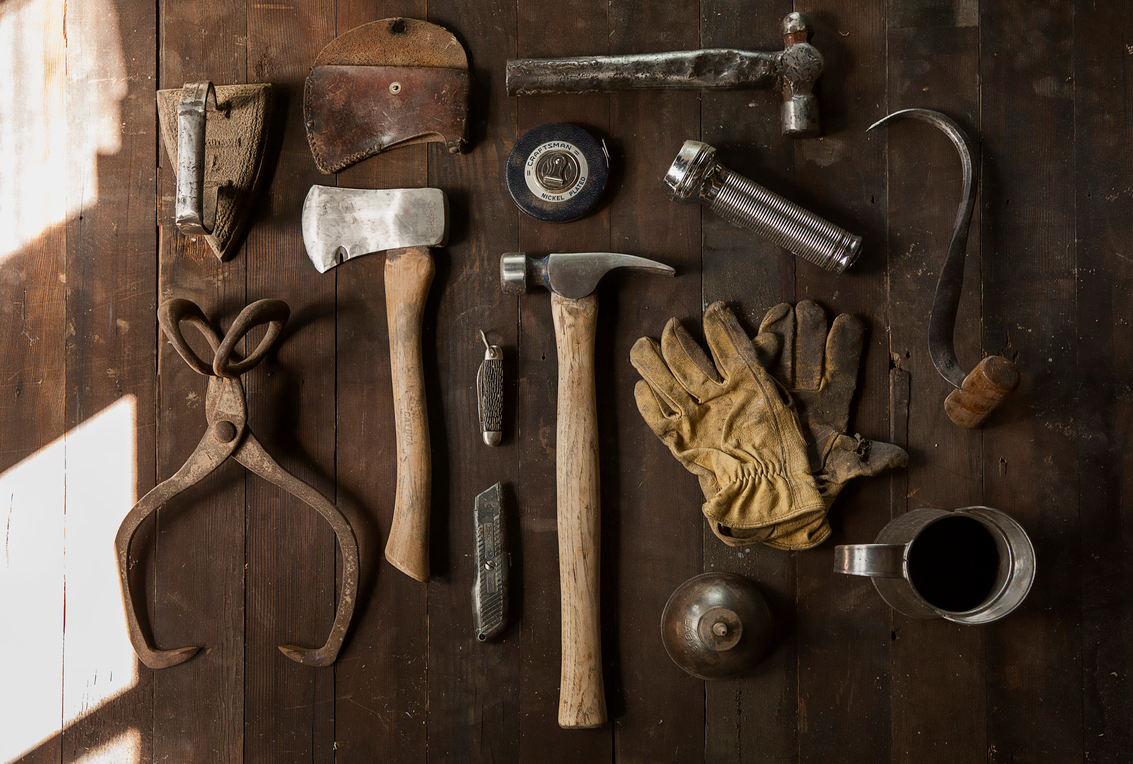
\includegraphics[width=\paperwidth]{images/Tools_by_Todd_Quackenbush.jpg}}
\setfootercentertext{
      \href{https://unsplash.com/@toddquackenbush?photo=IClZBVw5W5A}{
        https://unsplash.com/@toddquackenbush?photo=IClZBVw5W5A} - PD}
\begin{frame}
\end{frame}

\setbeamertemplate{background}{}
\setfootercentertext{}

\setfootercentertext{
  Mackinlay,  1986, \textit{ACM Transactions on Graphics},
  \href{https://doi.org/10.1145/22949.22950}{https://doi.org/10.1145/22949.22950}
}

\begin{frame}
  \frametitle{}
  \begin{center}
    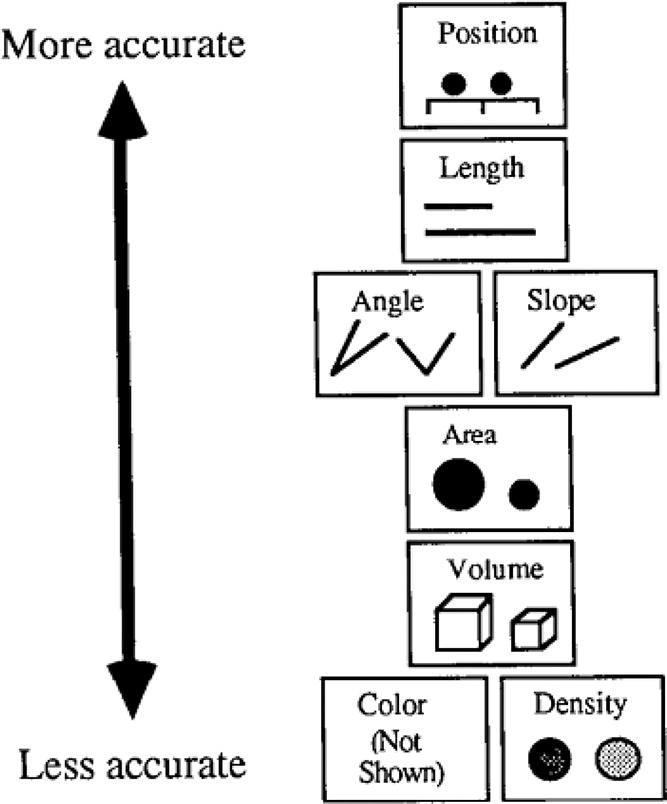
\includegraphics[width=5.0cm]{images/visualisation_accuracy.jpg}\\
  \end{center}
\end{frame}


\setbeamertemplate{background}{}
\setfootercentertext{}

\begin{frame}
  \frametitle{}
  \begin{center}
    {\Huge Live Coding }
  \end{center}
\end{frame}



\logo{}
\setbeamercolor{block body}{bg=lightgray}
\setbeamertemplate{background}{
  
\includegraphics[width=\paperwidth]{images/flickr_nateone_3768979925.jpg}}
\setfootercentertext{
  \href{https://www.flickr.com/photos/nateone/3768979925/}{https://www.flickr.com/photos/nateone/3768979925/}
  -- CC-BY by flick user
  \href{https://www.flickr.com/photos/nateone/}{nateone}}
\begin{frame}
  % \frametitle{Acknowledgements}
  \begin{block}{}
    \begin{center}
      \textbf{What are your questions?}\\
      \ \\
      \href{https://zbmed.de}{zbmed.de} / \href{https://twitter.com/ZB_MED}{@ZB\_MED} \\      
      \ \\
      \href{https://twitter.com/konradfoerstner}{@konradfoerstner}\\
      \ \\
      
\includegraphics[height=1.8cm]{images/ZBMED_2017_EN.pdf} 
      
\includegraphics[height=0.8cm]{images/logo_TH-Koeln_CMYK_22pt.eps}
      \\
    \end{center}
  \end{block}
\end{frame}

%%%%%%%%%%%%%%%%%%%%%%%%%%%%%
\section{Working on your data}
%%%%%%%%%%%%%%%%%%%%%%%%%%%%%

\setbeamertemplate{background}{}
\setfootercentertext{}

\begin{frame}{}
  \tableofcontents[currentsection]
\end{frame}


%%%%%%%%%%%%%%%%%%%%%%%%%%%%%
\section{Discussion, Questions \& Answers}
%%%%%%%%%%%%%%%%%%%%%%%%%%%%%

\begin{frame}{}
  \tableofcontents[currentsection]
\end{frame}

%%%%%%%%%%%%%%%%%%%%%%%%%%%%%
\section{Reading recommendations}
%%%%%%%%%%%%%%%%%%%%%%%%%%%%%


\begin{frame}
  \frametitle{Reading recommendations}
  \begin{block}{}  
    \begin{center}
      \begin{itemize}
      \item The
        \href{http://blogs.nature.com/methagora/2013/07/data-visualization-points-of-view.html}{\textit{Points
            of View}} Series in \textit{Nature Methods}
      \item \textit{Fundamentals of Data Visualization}, Claus Wilke,
        2019, O’Reilly Media, ISBN-13: 978-1492031086
      \item \textit{Visualization Analysis and Design}, Tamara
        Munzner, 2014, Taylor \& Francis, ISBN-13: 978-1466508910
      \end{itemize}
    \end{center}
  \end{block}    
\end{frame}

\end{document}
